% Dissertation roadmap (Chapter 1, sec:organization).
% Compile: pdflatex -output-directory=.. roadmap.tex
% Design: Palatino to match the thesis body, single arrow style, black
% outlines with near-white fills, dashed border for the future-work block.
% The feedback return enters the benchmark from the left margin so it clears
% every box; all labels sit in verified-empty zones.
\documentclass[border=6pt]{standalone}
\usepackage[T1]{fontenc}
\usepackage{mathpazo}
\usepackage{tikz}
\usetikzlibrary{arrows.meta, positioning, calc}
\begin{document}
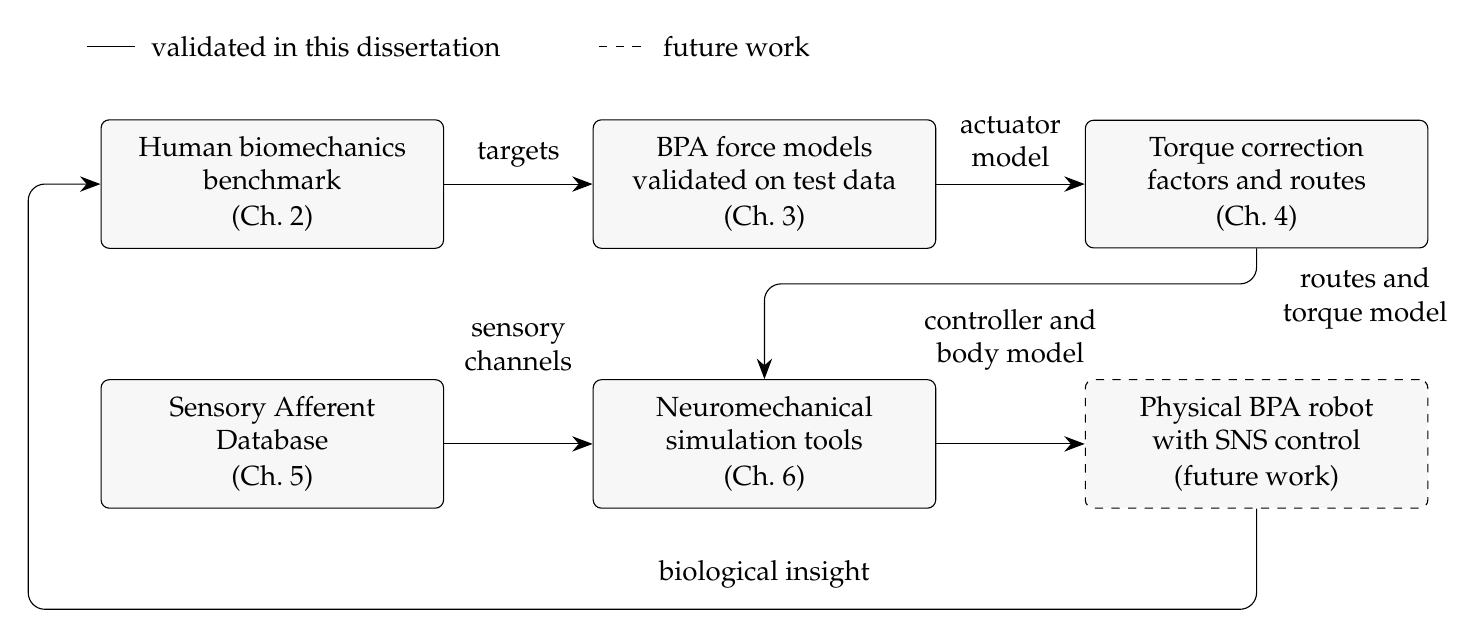
\begin{tikzpicture}[
  font=\normalsize,
  block/.style={draw, rounded corners=3pt, align=center, inner sep=6pt,
                minimum width=4.35cm, minimum height=1.5cm, fill=black!3},
  future/.style={block, dashed},
  arrow/.style={-{Stealth[length=2.6mm]}, thin, rounded corners=6pt},
  lab/.style={align=center, inner sep=3pt},
]

% Row 1
\node[block] (bench) at (0,0)      {Human biomechanics\\benchmark\\[1pt]{\normalsize (Ch.~2)}};
\node[block] (force) at (6.25,0)   {BPA force models\\validated on test data\\[1pt]{\normalsize (Ch.~3)}};
\node[block] (torq)  at (12.5,0)   {Torque correction\\factors and routes\\[1pt]{\normalsize (Ch.~4)}};
% Row 2
\node[block] (sadb)  at (0,-3.3)   {Sensory Afferent\\Database\\[1pt]{\normalsize (Ch.~5)}};
\node[block] (tools) at (6.25,-3.3){Neuromechanical\\simulation tools\\[1pt]{\normalsize (Ch.~6)}};
\node[future] (robot) at (12.5,-3.3){Physical BPA robot\\with SNS control\\[1pt]{\normalsize (future work)}};

% Row 1 arrows
\draw[arrow] (bench.east) -- node[lab, above=3pt] {targets} (force.west);
\draw[arrow] (force.east) -- node[lab, above=3pt] {actuator\\model} (torq.west);
% Torque down to the tools block; label pinned right of the drop
\draw[arrow] (torq.south) -- ++(0,-0.45) -| (tools.north);
\node[lab, anchor=west] at (12.72,-1.45) {routes and\\torque model};
% Row 2 arrows; labels set in the inter-row gap above the arrows
\draw[arrow] (sadb.east) -- (tools.west);
\node[lab, anchor=south] at (3.125,-2.48) {sensory\\channels};
\draw[arrow] (tools.east) -- (robot.west);
\node[lab, anchor=south] at (9.375,-2.48) {controller and\\body model};
% Feedback: robot to the left margin, up, into the benchmark from the west
\draw[arrow] (robot.south) -- (12.5,-5.4) -- (-3.1,-5.4) -- (-3.1,0) -- (bench.west);
\node[lab, anchor=south] at (6.25,-5.25) {biological insight};

% Key, spaced clear of all text
\draw[thin] (-2.35,1.75) -- (-1.75,1.75);
\node[lab, anchor=west] at (-1.65,1.75) {validated in this dissertation};
\draw[thin, dashed] (4.15,1.75) -- (4.75,1.75);
\node[lab, anchor=west] at (4.85,1.75) {future work};

\end{tikzpicture}
\end{document}
